% capitulo-2.tex
% Capítulo 2 — Antecedentes y trabajos relacionados
%
% Citations use the citation keys of the project Zotero library; the
% corresponding entries were exported to references.bib. Claims that would
% require a source not currently available in the library are marked with
% % TODO comments. Pending design decisions use visible \todo{...}
% placeholders (definidos en commands.tex, cargado desde main.tex).

\chapter{Antecedentes y trabajos relacionados}
\label{chap:background}

\section{Visión por computador en plataformas embebidas}
\label{sec:cv-embedded}

La visión por computador es la disciplina que se ocupa de extraer información
de imágenes y videos. Durante la última década, el enfoque dominante para
tareas como la clasificación de imágenes, la detección de objetos y la
segmentación ha transitado desde las características diseñadas manualmente
hacia las redes neuronales profundas, que aprenden representaciones visuales
directamente de los datos; este cambio es la premisa fundacional de la
literatura de aprendizaje profundo en el borde (\emph{edge deep learning})
\cite{xu2025}. La detección de objetos---la tarea de localizar y clasificar
múltiples objetos en una imagen--- es una primitiva de percepción canónica
para los sistemas robóticos, y comúnmente se realiza mediante detectores de
dos etapas, que primero proponen regiones candidatas y luego las clasifican,
o mediante detectores de una etapa, que predicen las detecciones directamente
a partir de mapas de características densos y en general sacrifican algo de
precisión a cambio de una mayor velocidad de procesamiento.
% TODO: cite a dedicated survey of deep-learning-based object detection
% covering the one-stage / two-stage taxonomy; no such survey is currently
% in the Zotero library. The edge benchmarking studies cited below use
% one-stage families exclusively.
En la práctica, las aplicaciones embebidas en tiempo real adoptan de manera
abrumadora las familias de detectores de una etapa, tales como YOLO, SSD y
EfficientDet, que son los sujetos estándar de los estudios de despliegue en
el borde \cite{alqahtani2026, szegedi2026, tang2026}.

Desplegar tales modelos a bordo de un robot o dispositivo autónomo impone
restricciones que no aplican al procesamiento fuera de línea o en centros de
datos. La cadena de procesamiento de percepción debe ejecutarse de manera
continua bajo plazos de tiempo real o casi tiempo real, dentro de límites
estrictos de potencia y temperatura, y con los recursos computacionales de
un procesador embebido en lugar de una estación de trabajo; la inferencia en
dispositivos de borde debe equilibrar simultáneamente velocidad, energía,
memoria, temperatura y precisión \cite{tang2026}. Para satisfacer estas
restricciones, los profesionales típicamente combinan tres ingredientes
\cite{xu2025, szegedi2026, tang2026}. Primero, arquitecturas de redes de
tamaño moderado o comprimidas: las familias de modelos se ofrecen en tamaños
graduados (p. ej., variantes que van de \emph{nano} a \emph{media}) y
técnicas como la destilación de conocimiento pueden comprimir un modelo
docente preciso en un estudiante adecuado para el borde, como se demostró
para la clasificación de imágenes médicas con despliegue en la propia Orin
Nano \cite{aalishah2025}. Segundo, precisión numérica reducida: la aritmética
FP16 e INT8 reduce la latencia, la huella de memoria y la energía a un costo
moderado en precisión \cite{szegedi2026, tang2026}. Tercero, entornos de
ejecución de inferencia optimizados por el fabricante que aprovechan los
aceleradores de GPU de la plataforma; en las plataformas Jetson, TensorRT
logra de manera consistente la latencia de inferencia más baja y una energía
sustancialmente menor por carga de trabajo que los frameworks no optimizados
\cite{szegedi2026, tang2026}.

De manera independiente del motor de inferencia, una aplicación de visión
por computador embebida presenta una estructura característica de cadena de
procesamiento: las imágenes se adquieren desde un sensor o se leen desde
almacenamiento, se preprocesan al formato esperado por el modelo, se pasan
por el modelo para la inferencia y se postprocesan para producir salidas a
nivel de aplicación, tales como cuadros delimitadores, etiquetas o imágenes
anotadas. Aunque la inferencia usualmente domina el presupuesto de cómputo,
las etapas circundantes no son despreciables: para cargas de trabajo de
detección de objetos, el preprocesamiento y el postprocesamiento representan
una porción sustancial del tiempo de ejecución total, especialmente a
resoluciones de entrada más altas o cuando la precisión reducida acelera la
inferencia \cite{szegedi2026}. Cada etapa puede ser, por lo tanto,
computacionalmente significativa, y la forma en que las etapas se
conectan---dentro de un proceso o a través de varios--- es precisamente la
pregunta arquitectónica que esta memoria investiga.

% TODO: fuente/atribución si la figura se reproduce de un trabajo publicado.
\begin{figure}[H]
  \centering
  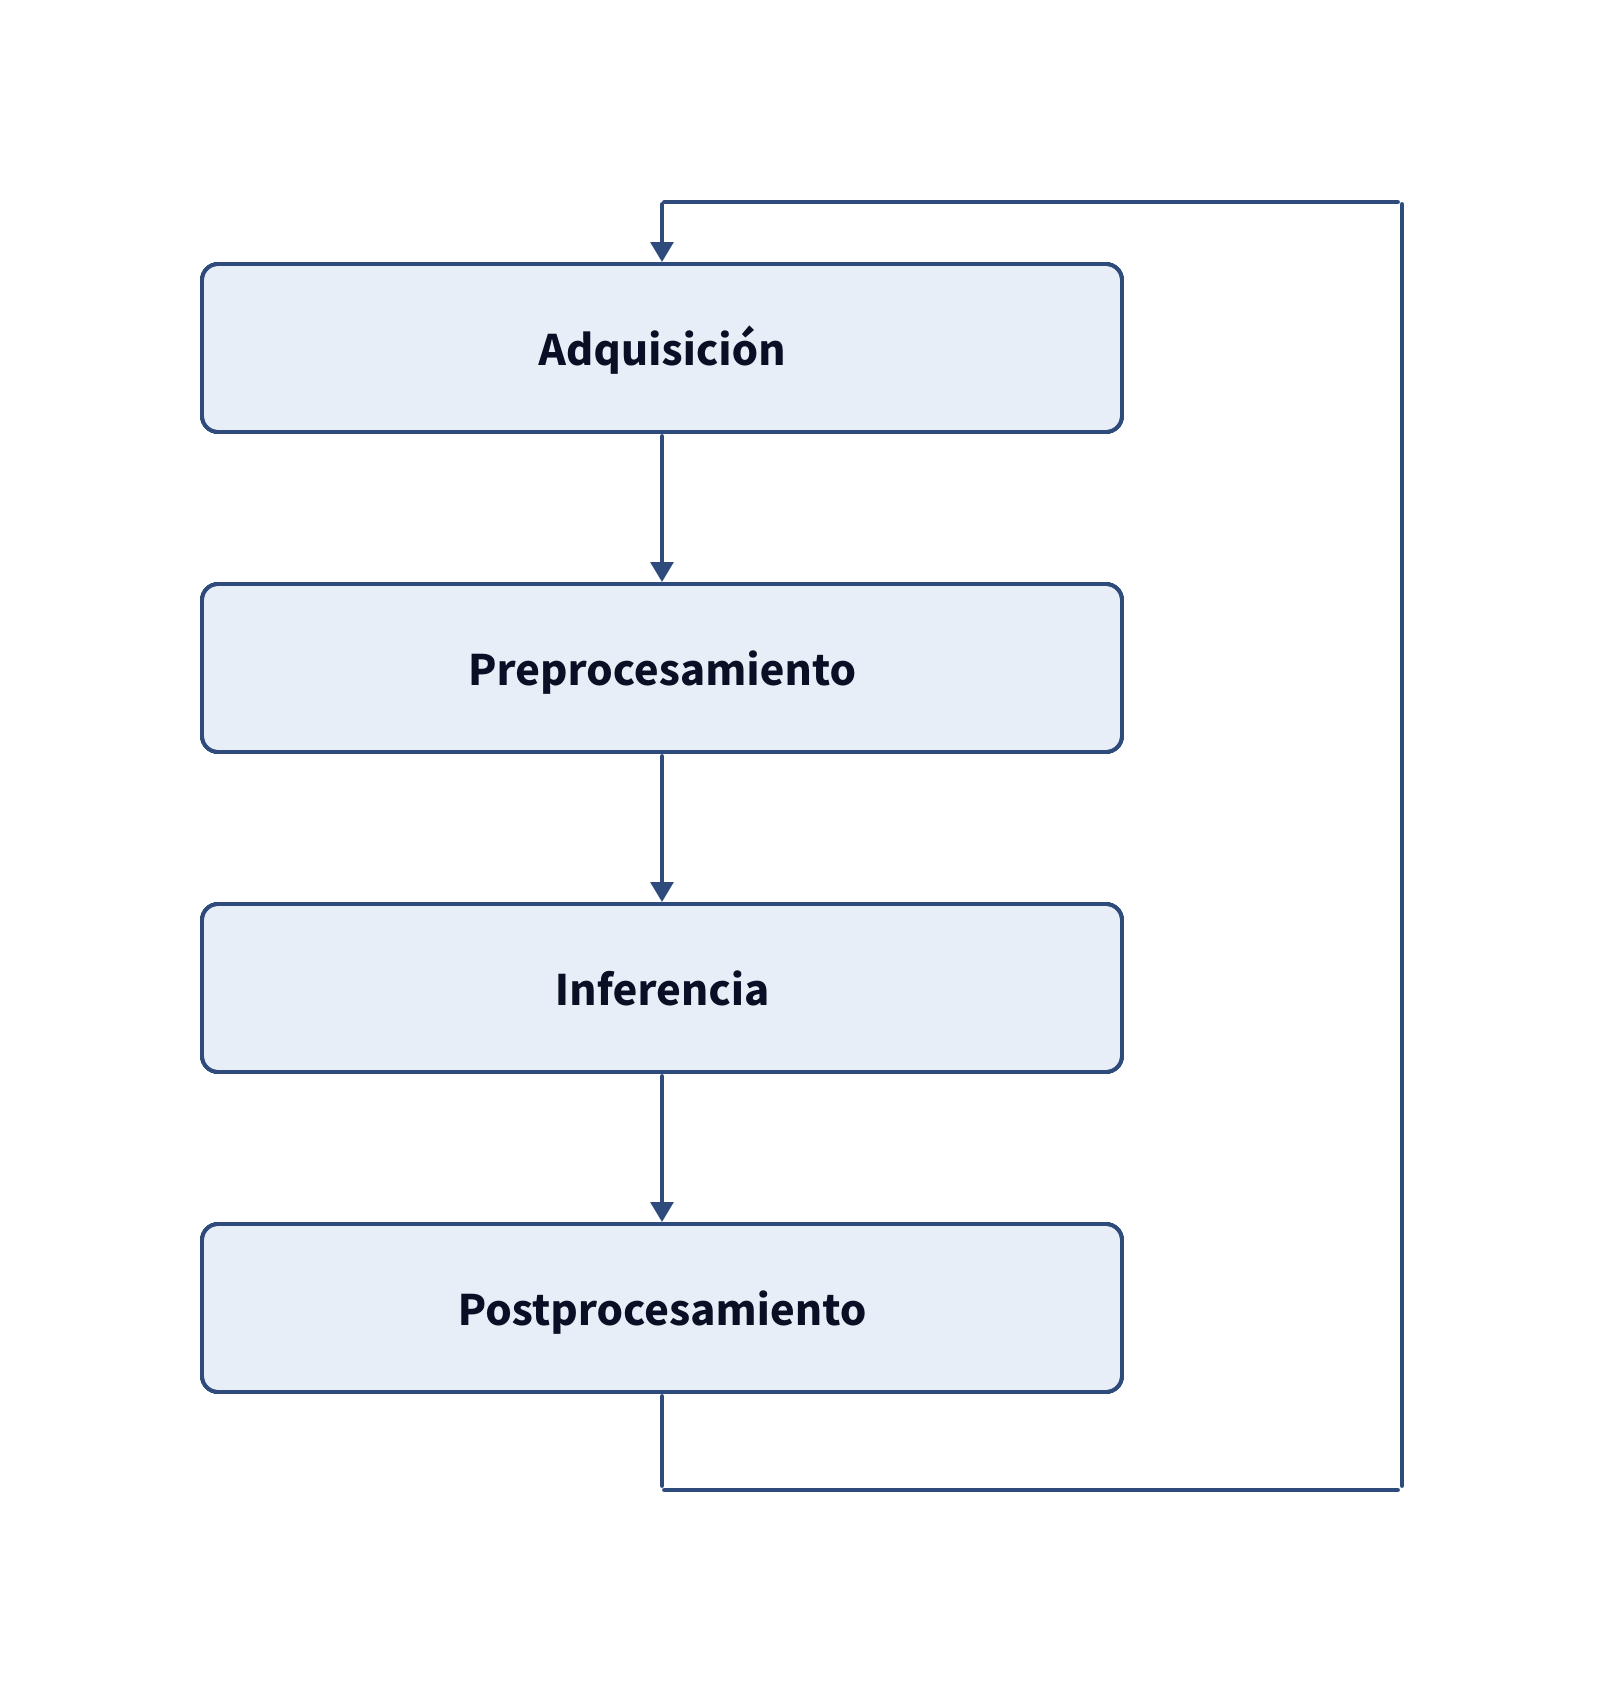
\includegraphics[height=0.5\textheight]{assets/figures/chapter-2/ciclo-CV.png}
  \caption[Cadena de procesamiento de visión por computador embebida.]{Cadena
  de procesamiento de visión por computador embebida. Las
  imágenes se adquieren desde un sensor o desde almacenamiento, se
  preprocesan al formato esperado por el modelo, se pasan por el modelo para
  la inferencia y se postprocesan para producir las salidas de la aplicación.
  La forma en que estas etapas se conectan (dentro de un único proceso o
  entre varios) es la variable arquitectónica bajo estudio en esta memoria.}
  \label{fig:cadena-vision-computador}
\end{figure}

\section{Arquitectura de NVIDIA Jetson}
\label{sec:jetson}

La familia NVIDIA Jetson comprende módulos de computación embebida que
integran núcleos de CPU Arm, una GPU de NVIDIA y memoria en una sola placa,
diseñados para cargas de trabajo de robótica e inteligencia artificial en
el borde \cite{scalcon2024}. Esta memoria utiliza la Jetson Orin Nano Super,
la configuración de kit de desarrollo (\emph{developer kit}) basada en el módulo
Jetson Orin Nano de 8~GB. Aquí se describen solo las características de
hardware relevantes para los experimentos; la configuración exacta del
módulo se documenta en el Capítulo~3.

\begin{figure}[H]
  \centering
  \figstub[0.5\linewidth]{assets/figures/chapter-2/jetson-orin-nano-module.jpg}
  \caption[Módulo NVIDIA Jetson Orin Nano.]{Módulo NVIDIA Jetson Orin
  Nano. El módulo integra en una única
  placa los núcleos de CPU Arm, la GPU de arquitectura Ampere con Tensor
  Cores y la memoria unificada; se monta sobre una placa portadora que expone
  los conectores de entrada y salida. Fotografía: NVIDIA Corporation.}
  \label{fig:jetson-orin-nano-module}
\end{figure}

El módulo se acopla a la placa portadora de referencia para formar el kit de
desarrollo (\Cref{fig:jetson-orin-nano-super-devkit}), que constituye
la plataforma sobre la cual se ejecutan los experimentos de esta memoria.

\begin{figure}[H]
  \centering
  \figstub[\linewidth]{assets/figures/chapter-2/jetson-orin-nano-super-devkit.jpg}
  \caption[Kit de desarrollo NVIDIA Jetson Orin Nano Super.]{Kit de
  desarrollo NVIDIA Jetson Orin Nano Super. El kit comprende
  el módulo Jetson Orin Nano de 8~GB montado sobre la placa portadora de
  referencia, con disipador y ventilador, y expone los conectores de entrada
  y salida utilizados en los experimentos: dos conectores de cámara MIPI
  CSI-2, cuatro puertos USB 3.2 Gen2 Tipo~A, Ethernet Gigabit, DisplayPort y
  ranuras M.2. Fotografía: NVIDIA Corporation.}
  \label{fig:jetson-orin-nano-super-devkit}
\end{figure}

El módulo Jetson Orin Nano de 8~GB combina una CPU Arm de seis núcleos
Cortex-A78AE con una GPU de NVIDIA de arquitectura Ampere que incluye 1024
núcleos CUDA y 32 Tensor Cores, las unidades dedicadas a las operaciones
matriciales aceleradas utilizadas en la inferencia de redes neuronales; su
rendimiento de inferencia alcanza hasta 67~TOPS \cite{nvidiacorporation2024}.
Una característica de la plataforma directamente relevante para este estudio
es su memoria física unificada: la CPU y la GPU acceden a la misma memoria
LPDDR5 de 8~GB, con un bus de 128~bits y un ancho de banda de 102~GB/s, en
lugar de memorias separadas de anfitrión y dispositivo
\cite{nvidiacorporation2024}.
Este diseño de memoria compartida influye en cuán costoso resulta mover
datos de imágenes entre etapas de procesamiento y entre procesos, lo cual es
uno de los costos introducidos al distribuir una cadena de procesamiento
entre múltiples procesos.

Dos características adicionales de la plataforma importan para la evaluación
comparativa de rendimiento reproducible. Primero, el módulo opera en modos
de energía seleccionables que comprometen rendimiento con consumo de
energía; el rango de potencia configurable del módulo va de 7~W a 25~W
\cite{nvidiacorporation2024}, y las evaluaciones publicadas de la familia
Orin distinguen explícitamente estas configuraciones---por ejemplo, la
configuración de 15~W de la Orin Nano--- al informar las tasas de fotogramas
alcanzables de análisis de video \cite{scalcon2024}, por lo que el modo de
energía debe fijarse y documentarse para todos los experimentos. Segundo,
las cargas de trabajo sostenidas están sujetas a efectos térmicos: bajo
carga de inferencia continua, la temperatura del dispositivo aumenta de
manera medible y debe monitorearse al caracterizar el rendimiento
\cite{tang2026}. La configuración de enfriamiento se fija y documenta, por
lo tanto, de la misma manera; el kit de desarrollo disipa el calor del
módulo mediante un disipador con ventilador \cite{nvidiacorporation2024}.

El entorno de software para las plataformas Jetson lo proporciona JetPack,
un paquete que incluye el sistema operativo Linux, las bibliotecas de
cómputo en GPU CUDA y bibliotecas de inferencia acelerada tales como
TensorRT \cite{szegedi2026, tang2026}. Las versiones exactas utilizadas en
esta memoria se registran en el Capítulo~3.

% TODO: fuente/atribución si el diagrama se adapta de la documentación de NVIDIA.
\begin{figure}[H]
  \centering
  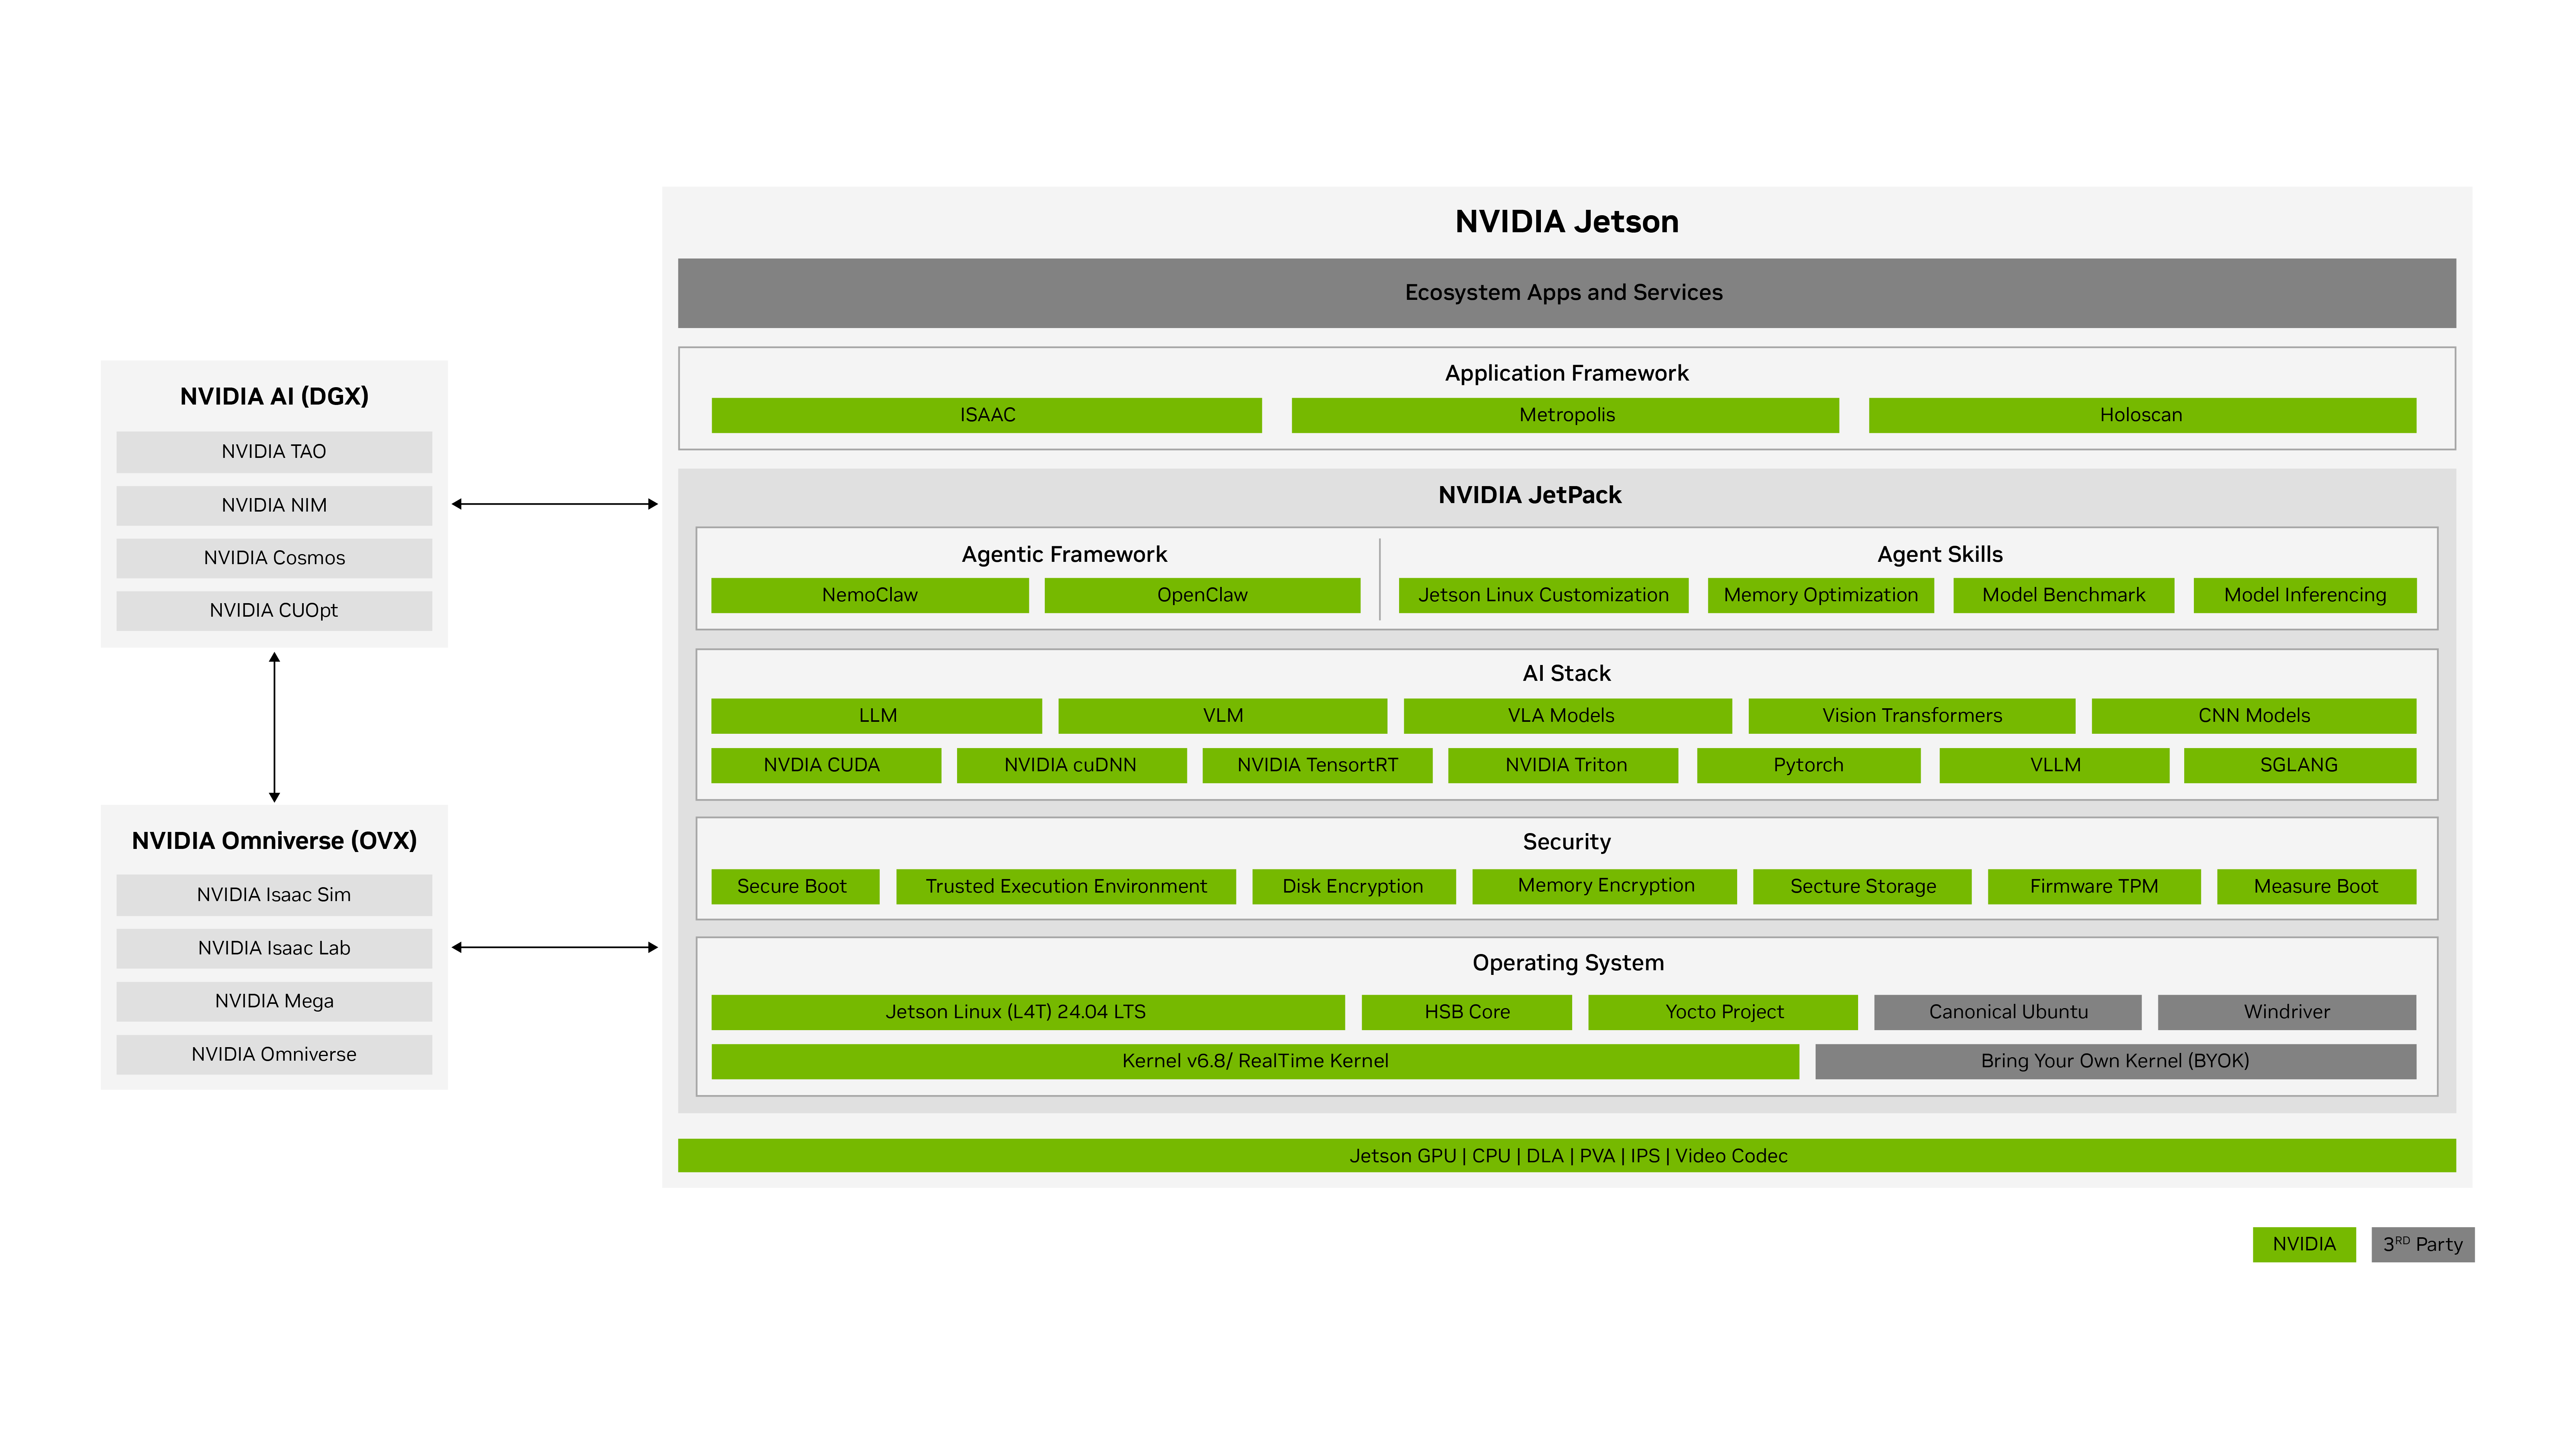
\includegraphics[width=\linewidth]{assets/figures/chapter-2/jetpack-stack.png}
  \caption[Stack de software de la plataforma Jetson.]{Stack
  de software de la plataforma Jetson. Sobre el
  SoC se disponen el sistema operativo Linux incluido en JetPack, las bibliotecas de
  cómputo en GPU (CUDA y bibliotecas asociadas) y las bibliotecas de
  inferencia acelerada como TensorRT, sobre las cuales se ejecuta la
  aplicación de visión por computador.}
  \label{fig:jetson-stack}
\end{figure}

\section{Arquitectura de ROS 2}
\label{sec:ros2}

ROS~2 es un framework de código abierto para desarrollar software de robots
como una colección distribuida de procesos cooperantes
\cite{macenski2022,rosjazzydocs}. Sus elementos arquitectónicos son los
nodos, los tópicos y los mensajes.

Un \emph{nodo} es un proceso que encapsula una pieza coherente de
funcionalidad, como leer una cámara, preprocesar imágenes o ejecutar un
modelo de red neuronal. Los nodos intercambian datos publicando y
suscribiéndose a \emph{tópicos}, que son buses nombrados que transportan
\emph{mensajes} tipados. Un nodo publicador escribe mensajes en un tópico y
cada nodo suscriptor a ese tópico recibe su propia copia del mensaje. Los
tipos de mensaje se definen de manera declarativa y existen tipos estándar
para los datos de imágenes utilizados por las aplicaciones de visión por
computador \cite{macenski2022, rosjazzydocs}.

% Fuente: ros2_documentation (rolling), archivo
% source/ROS-Framework/interfaces/topics/Understanding-ROS2-Topics/images/
% Topic-MultiplePublisherandMultipleSubscriber.gif; licencia CC BY 4.0.
% Adaptación: se eliminó el texto explicativo en inglés de la imagen original.
\begin{figure}[H]
  \centering
  \figstub{assets/figures/ros2-nodos-topico.png}
  \caption[Arquitectura basada en nodos de ROS~2.]{Arquitectura basada
  en nodos de ROS~2. Cada nodo encapsula una
  funcionalidad; los nodos intercambian datos publicando en tópicos nombrados
  y suscribiéndose a ellos. Un nodo publicador escribe un mensaje tipado en el
  tópico y cada nodo suscriptor recibe su propia copia de ese mensaje. Fuente:
  documentación oficial de ROS~2 (licencia CC BY 4.0), adaptada.}
  \label{fig:ros2-nodos-topico}
\end{figure}

Un nodo ejecuta la lógica de aplicación en \emph{callbacks} (funciones de
retrollamada): funciones invocadas en respuesta a eventos como la llegada de
un mensaje o la expiración de un temporizador. Los ejecutores
(\emph{executors}) son el mecanismo que toma los callbacks en cola y los
ejecuta. El modelo de ejecutores de ROS~2 ha sido analizado en detalle por
la comunidad de sistemas de tiempo real \cite{casini2026}: las
distribuciones estándar proporcionan un ejecutor de un solo hilo, que
procesa los callbacks secuencialmente dentro de un hilo; un ejecutor
multihilo, que puede ejecutar callbacks de manera concurrente; y una
variante estática de un solo hilo. La elección del ejecutor y la estructura
de los callbacks determinan cómo responde una etapa de la cadena de
procesamiento a los datos entrantes, y es imposible desacoplar el ejecutor
del rendimiento de un nodo \cite{macenski2023, casini2026}. La configuración
del ejecutor constituye, por lo tanto, parte de la configuración
arquitectónica bajo estudio.

% Fuente: ros2_documentation (rolling), archivo
% source/ROS-Framework/client-libraries/About-Executors/images/
% executors_basic_principle.png; licencia CC BY 4.0.
\begin{figure}[H]
  \centering
  \figstub[0.90\linewidth]{assets/figures/ros2-ejecutores-callbacks.png}
  \caption[Modelo de callbacks y ejecutores en ROS~2.]{Modelo de callbacks
  y ejecutores en ROS~2. Los callbacks se
  encolan al producirse un evento, como la llegada de un mensaje o la
  expiración de un temporizador, y el ejecutor se encarga de tomarlos de la
  cola y ejecutarlos. Un ejecutor de un solo hilo procesa los callbacks
  secuencialmente, mientras que un ejecutor multihilo puede ejecutarlos de
  manera concurrente. Fuente: documentación oficial de ROS~2 (licencia
  CC BY 4.0).}
  \label{fig:ros2-ejecutores-callbacks}
\end{figure}

ROS~2 ofrece varias bibliotecas cliente para diferentes lenguajes de
programación. Este trabajo utiliza rclpy, la biblioteca cliente de Python. La
mayoría de los usuarios interactúa con ROS~2 exclusivamente a través de tales
bibliotecas cliente, que proporcionan las APIs núcleo de comunicación y
descansan sobre capas inferiores comunes: una biblioteca intermedia en C,
rcl, que proporciona funcionalidad compartida por todas las bibliotecas
cliente, y por debajo de ella la capa de abstracción rmw (ROS MiddleWare), a
través de la cual se selecciona la implementación de comunicación
subyacente \cite{macenski2022, rosjazzydocs}. Esta estratificación es
relevante para la interpretación de las mediciones: el trabajo de perfilado
sobre la pila de C++ ha mostrado que una fracción significativa de la
latencia de extremo a extremo puede originarse por encima del transporte
mismo, en la ruta de notificación y recuperación entre el middleware y la
biblioteca cliente \cite{kronauer2021, kamiya2025}, de modo que el sobrecosto observado en una cadena de
ROS~2 en Python puede originarse en las capas de la biblioteca cliente y de
serialización, en lugar de en el transporte únicamente.

% Fuente: ros2_documentation (rolling), archivo
% source/ROS-Framework/client-libraries/About-Internal-Interfaces/images/
% ros_client_library_api_stack.png; licencia CC BY 4.0.
\begin{figure}[H]
  \centering
  \figstub[0.90\linewidth]{assets/figures/ros2-software-stack.png}
  \caption[Stack de software de ROS~2.]{Stack de software de ROS~2. Las
  aplicaciones se implementan sobre
  una biblioteca cliente según el lenguaje de programación (por ejemplo,
  rclpy para Python); todas las bibliotecas cliente comparten la biblioteca
  intermedia en C, rcl, y descansan sobre la capa de abstracción rmw, a través
  de la cual se selecciona la implementación de comunicación (middleware DDS)
  subyacente. Fuente: documentación oficial de ROS~2 (licencia CC BY 4.0).}
  \label{fig:ros2-software-stack}
\end{figure}

Finalmente, ROS~2 soporta nodos componibles: múltiples nodos cargados en un
único proceso, que pueden comunicarse mediante mecanismos intraproceso que
evitan la serialización y las copias \cite{macenski2023}. La composición es
el patrón de diseño recomendado de ROS~2 precisamente porque mitiga los
costos del modo multiproceso predeterminado \cite{macenski2022,macenski2023}.
Los nodos componibles quedan, sin embargo, explícitamente excluidos del
alcance de esta memoria (\Cref{sec:scope}): el objeto de estudio es la
arquitectura ordinaria de nodos multiproceso misma, y la composición se
discute como trabajo futuro en el Capítulo~6.

\section{Comunicación de ROS 2}
\label{sec:ros2-communication}

A nivel conceptual, ROS~2 delega la comunicación entre procesos a una
implementación del estándar Data Distribution Service (DDS), un middleware
de publicación--suscripción para sistemas distribuidos de tiempo real
\cite{gambo2025, macenski2022}. A diferencia de ROS~1, cuya comunicación
dependía de un máster central (\emph{rosmaster}), las implementaciones de
DDS descubren los pares automáticamente, emparejan publicadores con
suscriptores por tópico y tipo, e intercambian datos sin ningún agente
central \cite{macenski2022, gambo2025}. DDS es adecuado para sistemas
embebidos distribuidos de tiempo real debido a su comportamiento de
transporte configurable y su escalabilidad \cite{maruyama2016}, y el
middleware basado en DDS está hoy extendido en la robótica, respaldando
aplicaciones desde la coordinación multirobot hasta el procesamiento de
sensores en tiempo real \cite{gambo2025}.

Dos aspectos de este diseño son directamente relevantes para este trabajo.
Primero, DDS expone políticas de calidad de servicio (QoS) que determinan
las garantías de entrega y el comportamiento de almacenamiento en búfer: la
confiabilidad (\emph{best-effort} o \emph{reliable}), la durabilidad (p.
ej., \emph{volatile} frente a \emph{transient-local}), la configuración del
historial (colas \emph{keep-last} de una profundidad dada o \emph{keep-all})
y políticas adicionales como \emph{deadline}, \emph{lifespan} y
\emph{liveliness}, orientadas al diseño de sistemas de tiempo real
\cite{macenski2022,rosjazzydocs}. La configuración de QoS afecta de manera
medible la latencia y el uso de recursos: habilitar la entrega confiable y
las funciones de DDS-Security puede aumentar la latencia sustancialmente, y
una profundidad de historial reducida combinada con la entrega confiable
puede causar fallas de retransmisión \cite{fernandez2020,kronauer2021}. Por
esta razón, se utiliza una única configuración de QoS fija a lo largo de los
experimentos de esta memoria. Segundo, la capa de abstracción rmw permite
seleccionar diferentes implementaciones de DDS en tiempo de ejecución
\cite{maruyama2016, macenski2022}, y la elección afecta de manera medible el
rendimiento de la comunicación de forma dependiente del hardware
\cite{maruyama2016, kronauer2021, zhang2024}. La implementación se fija
igualmente para todos los experimentos, dado que comparar middlewares está
fuera del alcance de esta memoria.

Cuando un mensaje viaja entre dos nodos en procesos separados, atraviesa una
ruta que incluye la serialización del mensaje en una muestra del middleware,
su almacenamiento en la historia de escritura del publicador, el transporte
por sockets o memoria compartida, el almacenamiento en la historia de lectura
del suscriptor, la deserialización y, finalmente, la entrega del callback al
ejecutor. Tanto las historias de escritura y de lectura como el transporte son
gestionados por el middleware y no por el código del nodo \cite{rosjazzydocs};
cada paso consume tiempo y memoria, y cada uno ha sido cuantificado en la
literatura.

\begin{figure}[H]
  \centering
  \figstub{assets/figures/ros2-ruta-mensaje.png}
  \caption[Ruta de un mensaje entre dos nodos de ROS~2 en procesos separados.]{Ruta
  de un mensaje entre dos nodos de ROS~2 en procesos separados.
  El publicador serializa el mensaje en una muestra del middleware, que se
  almacena en la historia de escritura de su DataWriter (búfer de salida); el
  transporte la entrega a la historia de lectura del DataReader correspondiente
  (búfer de entrada). Ambas historias son mantenidas por el middleware y su
  tamaño y retención los fija la QoS, de modo que ni la profundidad efectiva
  del búfer ni la retención de muestras para suscriptores que se conectan
  tarde dependen del código del nodo. El suscriptor toma la muestra tras el
  aviso de disponibilidad que el middleware entrega a la biblioteca cliente,
  la deserializa en un mensaje ROS y la entrega al ejecutor como callback.
  Cada etapa consume tiempo y, para las cargas útiles grandes, contribuye de
  forma medible a la latencia total de la comunicación.}
  \label{fig:ros2-ruta-mensaje}
\end{figure} El perfilado de la pila de llamadas de ROS~2 muestra que
el sobrecosto con respecto a la comunicación DDS directa depende del tamaño
de la carga útil: para mensajes pequeños, la latencia está dominada por el
propio middleware DDS y por el retardo entre la notificación de DDS a la
biblioteca cliente y la recuperación efectiva de los datos por parte del
ejecutor, mientras que para cargas útiles grandes el transporte DDS domina
de manera absoluta \cite{kronauer2021}. Las mediciones resueltas por capa,
que registran marcas de tiempo en las fronteras entre las capas de ROS~2 y
DDS, atribuyen más de la mitad de la latencia total de la comunicación
predeterminada basada en sockets al segmento de transporte DDS, y muestran
que el transporte por memoria compartida reduce la latencia total a menos
de la mitad \cite{kamiya2025}. Incluso la comunicación intraproceso, que
pasa punteros en lugar de serializar, exhibe costos de publicación que crecen
con el tamaño del mensaje y con la cantidad de suscriptores que requieren
sus propias copias del mensaje \cite{luo2025}. Los mensajes grandes son
precisamente el punto débil de las configuraciones predeterminadas: los
tamaños de búfer UDP, la fragmentación de paquetes y las retransmisiones por
confiabilidad se combinan para degradar el rendimiento con cargas útiles del
orden de megabytes \cite{macenski2022, kronauer2021}--- y la propia
literatura de ROS~2 identifica las imágenes y las nubes de puntos como las
cargas útiles canónicas de este tamaño \cite{macenski2022, macenski2023}. Para los mensajes de imagen, cuyo
tamaño crece con la resolución, cabe esperar que el costo por mensaje de la
serialización y de las copias crezca en consecuencia; si esto se traduce en
una penalización medible de extremo a extremo a las resoluciones probadas es
una pregunta empírica que los experimentos de esta memoria están diseñados
para responder.

\section{Carga de trabajo de visión por computador}
\label{sec:workload}

La memoria utiliza una única carga de trabajo representativa de visión por
computador: una cadena de procesamiento de detección de objetos que procesa
un flujo de imágenes y produce detecciones con cuadros delimitadores. La
detección de objetos se eligió porque es una carga de trabajo de percepción
representativa y bien estudiada para la plataforma objetivo: las
evaluaciones publicadas demuestran la viabilidad de la detección de objetos
en tiempo real en la Orin Nano con modelos de las familias YOLO, SSD y
EfficientDet \cite{scalcon2024, alqahtani2026, szegedi2026, tang2026}. El
modelo de red neuronal exacto se seleccionará de acuerdo con los siguientes
criterios:

\begin{itemize}
  \item Capacidad de ejecutarse de manera confiable en la Jetson Orin Nano
  \item Reproducibilidad
  \item Disponibilidad de pesos del modelo documentados
  \item Tiempo de inferencia razonable
  \item Adecuación para procesamiento en tiempo real o casi tiempo real
\end{itemize}

\todo{SPECIFY: the final selected model, its source publication, weights
version, inference runtime, and any precision reduction applied. This
section must be completed once the model is chosen.}

El mismo modelo y la misma configuración de inferencia se utilizarán en cada
configuración de benchmark, de modo que la arquitectura de la aplicación sea
la única diferencia primaria entre las condiciones experimentales.

\section{Métricas de rendimiento}
\label{sec:metrics}

Esta sección define las métricas de rendimiento utilizadas en la memoria. El
conjunto sigue la práctica común de la literatura de rendimiento de ROS~2,
donde la latencia de extremo a extremo se descompone en componentes de
comunicación, cómputo e inactividad \cite{betz2023a} y se informa junto con
la tasa de procesamiento y la utilización de recursos
\cite{mayoral-vilches2024, macenski2022}.

\subsection{Latencia de extremo a extremo}

La latencia es el tiempo entre la entrada de un dato a la cadena de
procesamiento y la generación de la salida correspondiente---para las
cadenas de esta memoria, el tiempo transcurrido desde el momento en que un
fotograma se entrega a la primera etapa de procesamiento hasta que el
resultado completamente postprocesado de ese mismo fotograma está
disponible. La latencia es una cantidad distribucional: siguiendo la
práctica de los estudios de medición de ROS~2 \cite{kronauer2021,
macenski2022}, se resume mediante la media, la mediana, la desviación
estándar, el mínimo, el máximo y los percentiles 95 y 99 cuando hay muestras
suficientes. Los percentiles de la cola importan porque los resultados de
percepción que llegan tarde pueden ser tan inutilizables como aquellos que
nunca llegan \cite{betz2023a}.

\subsection{Tasa de procesamiento}

La tasa de procesamiento es la velocidad a la que los fotogramas completan
la cadena completa, medida en fotogramas por segundo (FPS), calculada como
fotogramas procesados dividido por el tiempo transcurrido.

\subsection{Utilización de CPU}

La utilización de CPU es la fracción de la capacidad de CPU en uso,
informada como utilización promedio y, donde sea útil, máxima, sobre el
intervalo de medición.

\subsection{Utilización de memoria}

La utilización de memoria es el uso de la RAM del sistema durante el
intervalo de medición; el uso de memoria de GPU también puede registrarse si
se dispone de una medición confiable.

\subsection{Utilización de GPU}

La utilización de GPU registra si el sobrecosto arquitectónico cambia la
utilización del recurso de cómputo principal para la inferencia.

\subsection{Consumo de energía (opcional)}

Si es posible una medición confiable y reproducible con el hardware
disponible, se registrarán las siguientes cantidades: potencia promedio,
potencia máxima, energía por fotograma procesado y rendimiento por vatio,
reflejando las métricas relacionadas con potencia utilizadas en los estudios
de caracterización de la Orin Nano \cite{tang2026}. La medición de potencia
se trata como una extensión opcional y no como un requisito.
% TODO: cite Jetson power-measurement methods (e.g., on-board power rails
% / tegrastats) if power measurement is included; official documentation
% is not currently in the library.

\section{Trabajos relacionados}
\label{sec:related-work}

La literatura relevante para esta memoria puede organizarse en cinco
categorías.

\paragraph{Benchmarks de comunicación de ROS~2.}
Una línea de trabajo evalúa de manera comparativa el rendimiento de la
comunicación del propio ROS~2. Maruyama et al.\ proporcionaron la
exploración sistemática más temprana, mostrando que las capas de ROS~2 sobre
DDS agregan sobrecosto y que la latencia de transporte varía con el tamaño
de los datos, la configuración y el proveedor de DDS \cite{maruyama2016}.
Kronauer et al.\ midieron la latencia de extremo a extremo en cadenas
multinodo de 3 a 23 nodos con tres middlewares DDS en un PC de escritorio y
una Raspberry Pi~4, perfilando la pila de llamadas y encontrando sobrecostos
de hasta 50\% con respecto a DDS puro para mensajes pequeños,
aproximadamente 30\% de pérdida de mensajes para cargas útiles de 500~KB en
el dispositivo embebido, y un crecimiento no lineal de la latencia más allá
de aproximadamente 13--17 nodos a tasas superiores a 50~Hz
\cite{kronauer2021}. Fernandez et al.\ cuantificaron el efecto de las
configuraciones de confiabilidad de QoS y de DDS-Security sobre la latencia
y la tasa de procesamiento \cite{fernandez2020}. Macenski et al.\ evalúan la
comunicación entre procesos, compuesta e intraproceso en la revisión de
diseño de ROS~2: con un publicador y un suscriptor, la latencia del
percentil 95 se mantiene por debajo de 1~ms para mensajes entre procesos de
hasta 1~MB, pero sube a 7,85~ms a 8~MB, con tasas sostenibles que caen de
1000~Hz a 213~Hz \cite{macenski2022}. Kamiya et al.\ instrumentaron las
fronteras internas de las capas de la comunicación por memoria compartida
\cite{kamiya2025}, y Luo et al.\ analizaron la escalabilidad de la
comunicación intraproceso, proponiendo la agrupación de mensajes
(\emph{message pooling}) para reducir los costos de asignación repetida
\cite{luo2025}. Estos estudios de microbenchmark caracterizan el middleware
con cargas útiles sintéticas y cadenas publicador--suscriptor,
predominantemente en C++; no integran el middleware en una aplicación de
extremo a extremo en la que la inferencia domina la carga de trabajo.

\paragraph{Estudios de middleware para robótica.}
La investigación más amplia sobre middleware enmarca a ROS~2 en su contexto.
Las revisiones sistemáticas mapean el rol del middleware basado en DDS en
las aplicaciones de robótica y sus desafíos abiertos, incluidos el
rendimiento y la escalabilidad \cite{gambo2025}, y las encuestas consolidan
los cambios arquitectónicos de ROS~1 a ROS~2 y el ecosistema construido
sobre ellos \cite{al-batati2026}, así como el soporte y el análisis de
tiempo real desarrollados para ROS~2 \cite{casini2026}. Zhang et al.\
comparan DDS contra los middlewares alternativos Zenoh y MQTT para la
comunicación de ROS~2 de borde a borde y de borde a la nube a través de
Ethernet, Wi-Fi y 4G, encontrando que la mejor elección depende de la red
\cite{zhang2024}. Portugal et al.\ encuestaron a la comunidad ROS sobre el
estado de la adopción de ROS~2, documentando tanto el cumplimiento de las
expectativas de los usuarios por parte del middleware como las razones que
retienen a los equipos de migrar \cite{portugal2025}. Estos estudios se
refieren a la selección y adopción de middleware y no a la arquitectura de
una aplicación única en un único anfitrión, que es el foco de este trabajo.

\paragraph{Benchmarks de visión por computador embebida.}
Otra línea de trabajo evalúa de manera comparativa la visión por computador
y la inferencia de aprendizaje profundo en plataformas embebidas. Alqahtani
et al.\ evaluaron nueve modelos de detección de objetos en dispositivos
Raspberry Pi con y sin aceleradores TPU, una Jetson Nano y una Jetson Orin
Nano, informando compromisos entre precisión, tiempo de inferencia y
energía, y encontrando que la Orin Nano ofrece el balance global más
favorable \cite{alqahtani2026}. Szegedi et al.\ compararon arquitecturas de
modelos, lenguajes de programación, frameworks de inferencia y precisiones
numéricas en una Orin Nano frente a una estación de trabajo de escritorio
\cite{szegedi2026}, y existen caracterizaciones comparables del
comportamiento de potencia, energía y temperatura bajo inferencia sostenida
\cite{tang2026}. Scalcon et al.\ evaluaron dispositivos de la familia Orin
para monitoreo de video con inteligencia artificial, informando la
utilización de CPU, GPU y RAM para una carga de trabajo de vigilancia
\cite{scalcon2024}. Más allá de los estudios de modelo único, el trabajo de
gestión de recursos examina el compartimiento de GPU entre aplicaciones
concurrentes de IA en el borde sobre hardware Jetson \cite{woo2025}, y el
diseño de modelos consciente del hardware apunta al despliegue eficiente en
la propia Orin Nano \cite{aalishah2025}. Estos estudios establecen el
rendimiento de inferencia alcanzable en la clase objetivo de dispositivos,
pero consideran la aplicación como un proceso único y por lo tanto no
abordan el costo del particionamiento arquitectónico.

\paragraph{Caracterización de la plataforma Jetson.}
Los estudios de esta categoría caracterizan las propias plataformas Jetson:
las tasas de fotogramas alcanzables de análisis de video entre modelos Orin
y configuraciones de potencia \cite{scalcon2024}, y el comportamiento de
potencia, energía y temperatura bajo carga sostenida de redes neuronales
\cite{tang2026}. Estos estudios informan los controles experimentales de
esta memoria---modo de energía fijo, configuración de enfriamiento fija,
calentamiento y monitoreo de temperatura--- más que su pregunta de
investigación de manera directa.

\paragraph{Sobrecosto de comunicación de ROS~2 en aplicaciones.}
La categoría más cercana a esta memoria comprende estudios que investigan el
sobrecosto que ROS~2 introduce en sistemas realistas. Macenski et al.\
evaluaron la composición de nodos en sistemas robóticos completos,
informando ahorros de 28\% de CPU y 33\% de RAM al componer una pila de
navegación completa en un proceso sobre ARM, y concluyendo que las cadenas
multiproceso a escala de imagen son prácticamente imposibles sin composición
\cite{macenski2023}. Betz et al.\ desarrollaron un flujo de trabajo de
evaluación para la pila de conducción autónoma de código abierto
Autoware.Universe, descomponiendo la latencia de extremo a extremo en
componentes de comunicación, cómputo e inactividad e identificando cuellos
de botella a través de configuraciones de software y hardware
\cite{betz2023a}, y más tarde evaluaron una variante de microservicios
contenerizados de la misma pila, encontrando mejoras de 5--8\% en la
latencia media de extremo a extremo respecto del despliegue directo sobre
Linux \cite{betz2024}. Adyacente a la robótica, la literatura de ingeniería
de software sobre arquitecturas monolíticas frente a microservicios reporta
que los monolitos superan en rendimiento a sus contrapartes microservicio en
una única máquina \cite{blinowski2022}, que la brecha de rendimiento es
medible y dependiente de la carga de trabajo \cite{tapia2020}, e incluso
identifica una tendencia de migrar de vuelta desde diseños distribuidos a
monolíticos por razones de costo, complejidad y rendimiento
\cite{felisberto2024}. Lo que ninguno de estos estudios proporciona es una
comparación en la que la carga de trabajo, el modelo, la entrada y el
hardware se mantienen equivalentes mientras que la arquitectura de la
aplicación misma es la variable bajo estudio, con una línea base de proceso
único, en una plataforma embebida, en Python.

\section{Vacío de investigación}
\label{sec:gap}

La literatura revisada puede resumirse por lo que cada línea deja sin
responder. Los microbenchmarks de middleware caracterizan la comunicación de
ROS~2 de forma aislada, con cargas útiles sintéticas y clientes
mayoritariamente en C++, pero no dentro de una cadena de visión completa en
la que la inferencia domina y enmarca los costos de comunicación
\cite{maruyama2016, kronauer2021, kamiya2025,luo2025, macenski2022}. Los
estudios de mitigación---composición, comunicación intraproceso,
transporte por memoria compartida, agrupación de mensajes---evalúan
alternativas a la arquitectura multiproceso y por lo tanto presuponen, en
lugar de medir, el costo de esa arquitectura frente a una línea base
monolítica \cite{macenski2023, kamiya2025, luo2025}. Los benchmarks de
inferencia en plataformas Jetson caracterizan el cómputo dominante pero
asumen una aplicación monolítica y dejan así inexplorada la dimensión de
comunicación \cite{szegedi2026, tang2026, alqahtani2026, scalcon2024}. Los
estudios de pila completa, como las evaluaciones de Autoware, miden
sistemas reales pero confunden innumerables factores algorítmicos y
arquitectónicos, sin una referencia equivalente de proceso único
\cite{betz2023a, betz2024}. La evidencia general sobre monolitos frente a
microservicios, por su parte, no es específica de la robótica y no involucra
ROS~2, cargas útiles de imagen ni hardware embebido \cite{tapia2020,
blinowski2022, felisberto2024}.

Lo que queda por caracterizar---y lo que esta memoria mide--- es el costo en
rendimiento de particionar una única cadena de procesamiento de visión por
computador en Python, funcionalmente equivalente, entre nodos rclpy de
ROS~2 en una única plataforma embebida, en función del grado de
particionamiento, bajo una implementación de DDS y una configuración de QoS
fijas, y con una metodología reproducible.
